\documentclass[border=0.2cm]{standalone}
 
% required packages and libraries
\usepackage{tikz}
\usetikzlibrary{automata, positioning}
 
\begin{document}
 
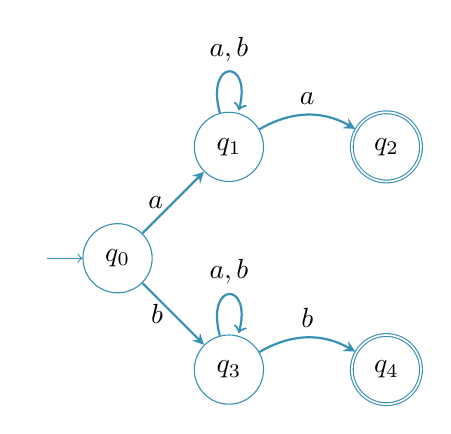
\begin{tikzpicture} [draw=cyan!70!black,
    node distance = 2cm, 
    on grid, 
    auto]
 
% State q0 
\node (q0) [state, 
    initial,  
    initial text = {}] {$q_0$};
 
% State q1    
\node (q1) [state, 
    above right = of q0] {$q_1$};

% State q2    
\node (q2) [state,
    accepting,
    right = of q1] {$q_2$};


% State q1    
\node (q3) [state, 
    below right = of q0] {$q_3$};

% State q2    
\node (q4) [state,
    accepting,
    right = of q3] {$q_4$};
 
% Arrows
\path [-stealth, thick]
    (q0) edge [left] node {$a$} (q1)
    (q0) edge [left] node {$b$} (q3)
    (q1) edge [bend left] node {$a$} (q2)
    (q3) edge [bend left] node {$b$} (q4)

	(q1) edge [loop above]  node {$a,b$}()
	(q3) edge [loop above]  node {$a,b$}()
    ;
\end{tikzpicture}
 
\end{document}